\documentclass[11pt,a4paper,titlepage]{article}
\usepackage[utf8]{inputenc}
\usepackage[english]{babel}
\usepackage[T1]{fontenc}

\RequirePackage[layout=inline]{fixme}

\usepackage{float}
\usepackage{graphicx}
\usepackage{setspace}
\usepackage{amsmath}
\usepackage{courier}
\usepackage{amsmath}
\usepackage{listings}
\usepackage{color}
\usepackage[toc, page]{appendix}

\usepackage{algpseudocode}
\usepackage[bottom]{footmisc}
\usepackage{verbatimbox}

\usepackage{changepage}

\usepackage{multirow}


\definecolor{mygreen}{rgb}{0,0.6,0}
\definecolor{mygray}{rgb}{0.5,0.5,0.5}
\definecolor{mymauve}{rgb}{0.58,0,0.82}


%% Units:
\newcommand{\W}{\,\textrm{W}}
\newcommand{\A}{\,\textrm{A}}
\newcommand{\mA}{\,\textrm{mA}}
\newcommand{\N}{\,\textrm{N}}
\newcommand{\Hz}{\,\textrm{Hz}}
\newcommand{\V}{\,\textrm{V}}
\newcommand{\Ohms}{\,\Omega}
\newcommand{\kOhm}{\,\text{k}\Omega}
\newcommand{\nF}{\,\textrm{nF}}
\newcommand{\dB}{\,\textrm{dB}}
\newcommand{\VperBit}{\,\textrm{V/bit}}
\newcommand{\NperBit}{\,\textrm{N/bit}}

\newcommand{\degC}{\,^{\circ}\text{C}}

\lstset{ %
	backgroundcolor=\color{white},   % choose the background color
	basicstyle=\scriptsize,        % size of fonts used for the code
	breaklines=true,                 % automatic line breaking only at whitespace
	captionpos=b,                    % sets the caption-position to bottom
	commentstyle=\color{mygreen},    % comment style
	escapeinside={\%*}{*)},          % if you want to add LaTeX within your code
	keywordstyle=\color{blue},       % keyword style
	stringstyle=\color{mymauve},     % string literal style
	numbers=left,
}

%\renewcommand{\thesubsection}{\thesection.\alph{subsection}}



\usepackage{booktabs}
\usepackage[backend=biber, bibencoding=utf8, style=ieee]{biblatex}

\addbibresource{references.bib}
\usepackage[final,hidelinks]{hyperref} % must be last package loaded

\author{Ólafur Jón Thoroddsen}  % My name, for the titlepage
\title{\includegraphics{graphics/ru-logo}\\\vspace{10mm}
	Mechatronics II\\T-535-MECH \ \\Homework 9}  % The title, for the titlepage

\begin{document}
	\pagenumbering{arabic}
	\maketitle
	
	\tableofcontents
	\pagebreak
	
	\section{Vishay SI4384DY fast switching MOSFET}
	
	The SI4384DY is the transistor that the Arduino board uses for motor control. From the datasheet~\cite{si4384dy} for the SI4384DY we have the thermal resistance ratings as shown in table~\ref{tab:thermal}.
	
	\begin{table}[h]
		\centering
		\hspace*{-2.7cm}
		\begin{tabular}{lccccc}
			\toprule
			\textbf{Parameter}	&	&	\textbf{Symbol}	&	\textbf{Typical}	&	\textbf{Maximum}	&	\textbf{Unit}\\
			\midrule
			Maximum Junction-to-Ambient (MOSFET)	&	Steady State	&	$\text{R}_{\text{thJA}}$	&	71	&	85	&	$\degC$/W\\	
			\bottomrule
		\end{tabular}
		\caption{Thermal resistance rating for the SI4384DY transistor}
		\label{tab:thermal}
	\end{table}
	\vspace{5mm}
	
	\noindent The resistance from drain to source ($\text{R}_{\text{DS}}$) in the transistor is dependent on the gate to source voltage ($\text{V}_{\text{GS}}$). The datasheet provides two values for $\text{R}_{\text{DS}}$, shown in table~\ref{tab:rds}.
	
	\vspace{5mm}
	\begin{table}[h]
		\centering
		\begin{tabular}{clc}
			\toprule
			$\textbf{V}_{\textbf{DS}}$	[V]	&	$\textbf{R}_{\textbf{DS}}$ [$\Omega$]	&	$\textbf{I}_{\textbf{D}}$ [A]\\
			\midrule
			\multirow{2}{*}{30} 	&		0.0085 at $\text{V}_{\text{GS}} = 10\V$	&	15\\
			&	0.0125 at $\text{V}_{\text{GS}} = 4.5\V$	&	12\\
			\bottomrule
		\end{tabular}
		\caption{The resistance values of the Drain-Source path through the transistor for different values of $\text{V}_{\text{GS}}$.}
		\label{tab:rds}
	\end{table}
	\vspace{5mm}
	
	\noindent The Arduino's logic voltage is 5\V\ so $\text{R}_{\text{DS}} \approx 0.0125~\Omega$. If a motor is connected to the transistor and $\text{I}_\text{D} = 10\A$, the power dissipation is 
	\begin{equation}
	\begin{aligned}
		P &= I_D^2R_{DS} \\
		&= 10^2 \times 0.0125\\
		&= 1.25\W\\
	\end{aligned}
	\end{equation} 	
	
	\noindent From table~\ref{tab:thermal}, the Junction-to-Ambient temperature is then
	\[
		T = 71\times 1.25 = 88.75\degC
	\]
	
	
	\section{Analog-Digital Converters (ADCs)}
	
	There are a lot of different ways that an analog signal can be converted into a digital signal. Three ways discussed here are: Dual slope ADCs, Flash ADCs and Successive Approximation Register ADCs (SAR ADCs).
	
	\subsection{Dual Slope ADCs}
	The idea with Dual Slope ADCs is to charge a capacitor for a fixed amount of time and then discharge it with a constant current for a variable amount of time. The discharge time, which is proportional to the input voltage, is measured and converted to a binary number, representing the input voltage. Figure~\ref{fig:dualslope} shows a simple integrating circuit that could be the heart of such an ADC. The capacitor would actually be charged using a constant current source that depends on $V_{\textsc{in}}$ but not directly using $V_{\textsc{in}}$ as shown here. The switching between $V_{\textsc{in}}$ and $V_{\textsc{ref}}$ would be implemented in microcontroller logic or using a transistor circuit.
	
	\begin{figure}[h]
		\centering
		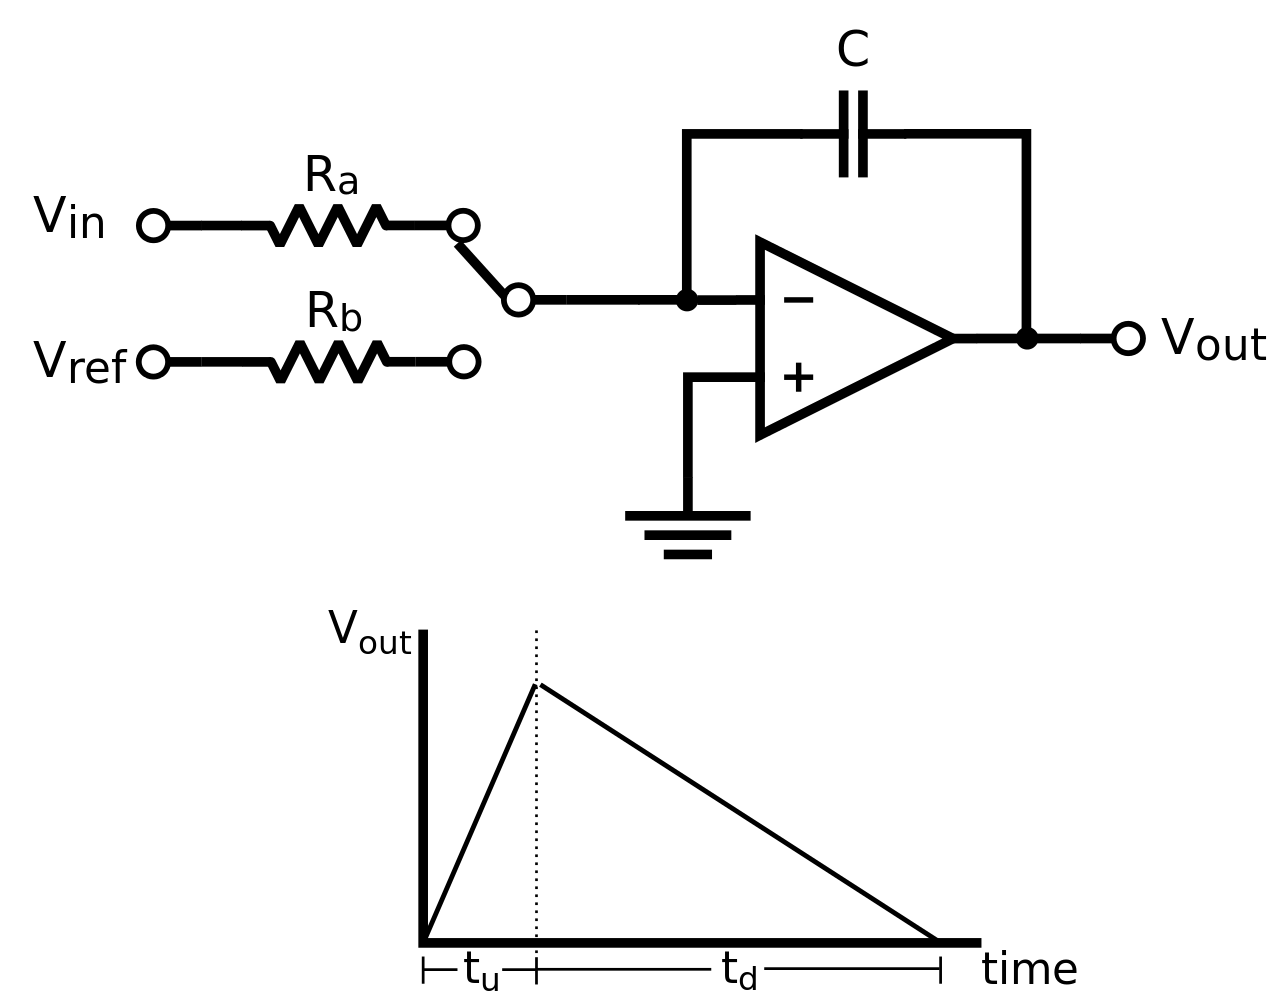
\includegraphics[width=\textwidth]{graphics/dualslope}
		\caption{A simple integrating circuit along with it's voltage/time characteristics~\cite{dualslope}.}
		\label{fig:dualslope}
	\end{figure}
	
	\begin{itemize}
		\item[Pros:]
		\begin{itemize}
			\item This kind of ADC is rather inexpensive to manufacture.
			\item Only a few components are needed, a capacitor, resistances and an op-amp. The timing can then be taken care of by a microcontroller (assuming that this is not a self-contained device). 
			\item Up to 14 bits of resolution.
		\end{itemize}
		\item[Cons:]
		\begin{itemize}
			\item Conversion time can be up to a few milliseconds. That is not always a problem but it can be in some applications.
		\end{itemize}
	\end{itemize}
	
	\noindent An example of a good application for a dual slope ADC is in a digital multimeter. The high resolution can give accurate results and it is not a problem though the conversion takes a few or even tens of milliseconds.
	
	
	\subsection{Flash ADCs}
	Flash ADCs are comprised of cascaded comparators, all connected to the same reference voltage $V_{\textsc{REF}}$ through a different combination of resistors. This results in a circuit that fires off a different number of comparators depending on the input voltage. The comparator outputs are then fed into a digital logic encoder which outputs the actual bit pattern representing the input voltage. Figure~\ref{fig:flashadc} shows the architecture of an arbitrarily large Flash ADC.
	
	\begin{figure}[H]
		\centering
		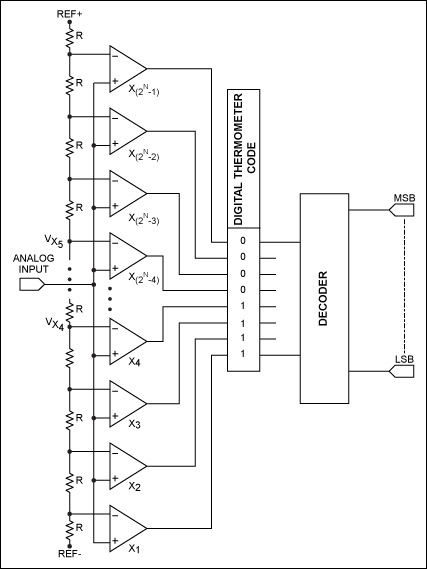
\includegraphics[width=0.7\textwidth]{graphics/flashadc}
		\caption{The architecture of a Flash ADC. The complexity increases rapidly with higher resolution~\cite{flashadc}}
		\label{fig:flashadc}
	\end{figure}
	
	\begin{itemize}
		\item[Pros:]
		\begin{itemize}
			\item Extremely fast, no need to wait for a capacitor to charge and discharge or anything like that.
		\end{itemize}
		\item[Cons:]
		\begin{itemize}
			\item The complexity of the circuit increases by a factor of 2 each time a single bit of resolution is added. For an \textit{N}-bit Flash ADC, $2^N - 1$ comparators are needed.
			\item Flash ADCs are more expensive then most other ADC architectures.
			\item Accuracy is seldom higher then 8-bits, because of the two previously mentioned points.
		\end{itemize}
	\end{itemize}
	
	\noindent While the Flash ADC is expensive and requires a large circuit to work, it is used in very high performance applications, for example in laboratory oscilloscopes where accuracy and sampling rate are valued somewhat more then cost. Tricks can be used to create for example an 8-bit Flash ADC from two 4-bit Flash ADCs using the implementation shown in figure~\ref{fig:halfflashadc}. This way, the overall number of comparators can be reduced from 255 to 30.
	
	\begin{figure}[H]
		\centering
		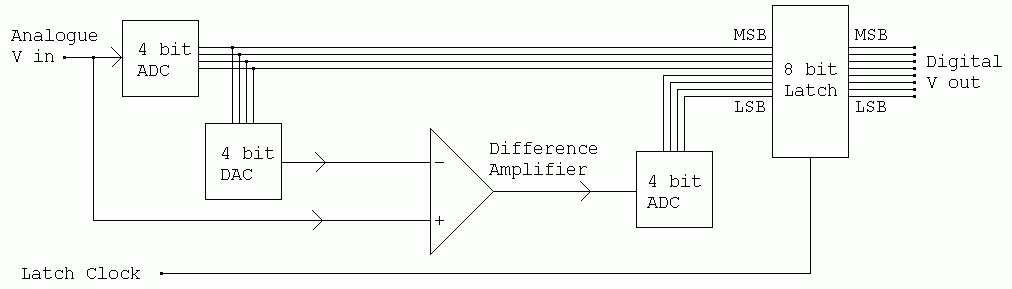
\includegraphics[width=\textwidth]{graphics/halfflashadc}
		\caption{The architecture of an 8-bit half flash ADC~\cite{halfflash}}
		\label{fig:halfflashadc}
	\end{figure}
	
	\subsection{Successive Approximation Register (SAR) ADCs}
	SAR ADCs use binary search to look for the bit pattern that represents the input voltage.
	Figure~\ref{fig:saradc} shows a diagram of a simple SAR ADC.
	A reference voltage $V_{\textsc{REF}}$ is fed into a comparator whose other input is the voltage being converted $V_{\textsc{in}}$.
	First, the reference voltage is set to be half way between the supply voltage and ground.
	The comparator then tells whether $V_{\textsc{in}}$ > $V_{\textsc{REF}}$ or $V_{\textsc{in}}$ < $V_{\textsc{REF}}$.
	The result is then used to adjust $V_{\textsc{REF}}$ to move closer to $V_{\textsc{in}}$.
	
	\begin{figure}[H]
		\centering
		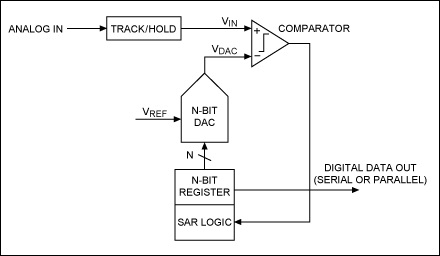
\includegraphics[width=0.9\textwidth]{graphics/saradc}
		\caption{Simplified diagram of a SAR ADC architecture~\cite{saradc}.}
		\label{fig:saradc}
	\end{figure}
	
	\begin{itemize}
		\item[Pros:]
		\begin{itemize}
			\item Great performance-cost ratio
			\item Internal elements can be inexpensive to manufacture
			\item High resolution converters are fairly easily implemented.
		\end{itemize}
		\item[Cons:]
		\begin{itemize}
			\item Higher resolution require that the accuracy of the internal components is very high.
			\item Sampling rate is limited because each bit takes "a single timestep" in contrast to for example the Flash ADC where all \textit{N} bits are converted in a single step. This is somewhat like the difference between serial and parallel communication.
		\end{itemize}
	\end{itemize}
	
	
	\noindent Overall the SAR ADCs provide a great performance for most general purpose applications. Most microcontrollers (including the ATmega328p) use a SAR ADC for interfacing with analog signals. If there is not a specific need for extremely high speed or extremely high accuracy, the SAR is a good choice.
	
	
	\section{Creating negative voltage from a positive power supply}
	
	Some devices require a supply voltage $V_{\textsc{cc}}$ as well as the negative of that voltage to operate. Voltage is of course always relative to some reference point and to generate a negative voltage, that reference point, the ground (\textsc{gnd}) needs to be midway between the power supply's highest voltage and lowest voltage.
	
	Figure~\ref{fig:negvolt} shows how this new reference point can be created from $V_{\textsc{cc}}$ by using a voltage divider. The output of the buffer becomes a virtual ground and the positive and negative voltages become $V_{\textsc{cc}}/2$ and $-V_{\textsc{cc}}/2$.
	
	\begin{figure}[H]
		\centering
		\includegraphics[width=0.7\textwidth]{graphics/VoltageDivider}
		\caption{A voltage divider creating a new reference point at $V_{\textsc{cc}}/2$}
		\label{fig:negvolt}
	\end{figure}
	
	
	\pagebreak
	\section{Progress with my project}
	
	\subsection{Last week}
	
	
	

	\subsection{Next week}
	
	\begin{table}[h]
		\centering
		\begin{tabular}{llc}
			\toprule
			Task no.	&	Task	&	ETC\footnotemark\\
			\midrule
			1	&	\begin{tabular}{@{}l@{}}Finish the IMU module\\\end{tabular} &	5 hours \\	
			\midrule	
			2	&	\begin{tabular}{@{}l@{}}Write the PWM code that uses output compare pins\end{tabular}	&	10 hours\\
			\midrule
			3	&	\begin{tabular}{@{}l@{}}Test the accuracy of the\\IMU sensor\end{tabular}	&	5 hours\\
			\midrule
			4	&		\begin{tabular}{@{}l@{}}Plan the control system and\\start designing at a high level\end{tabular}	&	5 hours\\
			\bottomrule
		\end{tabular}
		\label{tab:nextweek}
	\end{table}
	
	
	\footnotetext{Estimated Time to Complete}

	\subsection{Long term plan}
	
	\begin{table}[h]
		\centering
		\hspace*{-2cm}
		\begin{tabular}{lccc}
			\toprule
			Week	&	Software design	&	Mechanical design	&	Testing\\
			\midrule
			9	&	IMU \& PWM	&	\begin{tabular}{@{}l@{}}Power circuitry\\2nd prototype\end{tabular}	&	\begin{tabular}{@{}l@{}}Estimate power consumption\\PID motor control\end{tabular}\\
			\midrule
			10	&	Rethink PID control	&	3D drawing of the robot	&	Power consumption	\\
			\midrule
			11	&	\begin{tabular}{@{}l@{}}Integrate IMU, PID\\ and PWM modules\end{tabular}	&	Altium schematics of electronics	&	Integration\\
			\midrule
			12	&	Integration	&	Integration	&	Integration	\\
			\bottomrule
		\end{tabular}
		\label{tab:longterm}
		\hspace*{-2cm}
	\end{table}
	
	
	
\pagebreak
%\section*{Appendices}
\appendix



\pagebreak
\printbibliography

\end{document}